\subsubsection{list\_data::ListData}

\label{list_data::ListData}
\begin{figure}[ht]
	\centering
	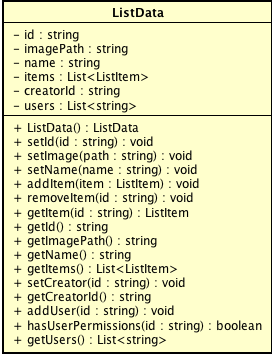
\includegraphics[scale=0.5]{Sezioni/SottosezioniST/img/app/ListData.png}
	\caption{list\_data::ListData}
\end{figure}

\begin{itemize}
\item \textbf{Descrizione}: Questa classe rappresenta la lista-spesa.
\item \textbf{Utilizzo}: Viene utilizzata da tutte le classi che hanno a che fare con la lista, ovvero che creano, modificano e rimuovono liste, o che aggiungono o rimuovono utenti e oggetti al suo interno.
\item \textbf{Attributi}: 
	\begin{itemize}
	\item \textit{private id:string}\\
	Questa stringa rappresenta l'identificativo della lista.
	\item \textit{private imagePath:string}\\
	Questa stringa rappresenta il percorso dell'immagine della lista.
	\item \textit{private name:string}\\
	Questa stringa rappresenta il nome della lista.
	\item \textit{private items:List<ListItem>}\\
	La lista degli oggetti contenuti dalla lista.
	\item \textit{private creatorId:string}\\
	Questa stringa rappresenta l'identificativo del creatore della lista.
	\item \textit{private users:List<string>}\\
	La lista degli identificativi di tutti i partecipanti alla lista-spesa.
	\end{itemize}
\item \textbf{Metodi}:
	\begin{itemize}
	\item \textit{public ListData():ListData}\\
	Il costruttore della classe ListData.
	\item \textit{public setId(id:string):void}\\
	Imposta l'id della lista.
				\item{\textbf{Parametri}: \begin{itemize}
				\item \textit{id:string}\\
				L'id che verrà impostato per la lista.
			\end{itemize}}
	\item \textit{public setImage(path:string):void}\\
	Imposta l'immagine della lista.
				\item{\textbf{Parametri}: \begin{itemize}
				\item \textit{path:string}\\
				Il percorso dell'immagine che verrà impostata per la lista.
			\end{itemize}}
	\item \textit{public setName(name:string):void}\\
	Imposta il nome della lista.
				\item{\textbf{Parametri}: \begin{itemize}
				\item \textit{name:string}\\
				Il nome che verrà impostato per la lista.
			\end{itemize}}
	\item \textit{public addItem(item:ListItem):void}\\
	Aggiunge un oggetto alla lista.
				\item{\textbf{Parametri}: \begin{itemize}
				\item \textit{item:ListItem}\\
				L'oggetto che verrò aggiunto alla lista.
			\end{itemize}}
	\item \textit{public removeItem(id:string):void}\\
	Rimuove un oggetto dalla lista.
				\item{\textbf{Parametri}: \begin{itemize}
				\item \textit{id:string}\\
				L'identificativo dell'oggetto che si desidera rimuovere dalla lista.
			\end{itemize}}
	\item \textit{public getItem(id:string):void}\\
	Ritorna un oggetto della lista.
				\item{\textbf{Parametri}: \begin{itemize}
				\item \textit{id:string}\\
				L'identificativo dell'oggetto che si desidera.
			\end{itemize}}
	\item \textit{public getId():string}\\
	Ritorna l'identificativo della lista.
	\item \textit{public getImagePath():string}\\
	Ritorna il percorso dell'immagine della lista.
	\item \textit{public getName():string}\\
	Ritorna il nome della lista.
	\item \textit{public getItems():List<ListItem>}\\
	Ritorna una lista contenente tutti gli oggetti presenti all'interno della lista.
	\item \textit{public setCreator(id:string):void}\\
	Imposta il creatore della lista.
				\item{\textbf{Parametri}: \begin{itemize}
				\item \textit{id:string}\\
				L'identificativo dell'utente che verrà impostato come creatore della lista.
			\end{itemize}}
	\item \textit{public getCreatorId():string}\\
	Ritorna l'identificativo del creatore della lista.
	\item \textit{public addUser(id:string):void}\\
	Aggiunge un utente ai partecipanti della lista.
				\item{\textbf{Parametri}: \begin{itemize}
				\item \textit{id:string}\\
				L'identificativo dell'utente che si desidera aggiungere alla lista.
			\end{itemize}}
	\item \textit{public hasUserPermissions(id:string):boolean}\\
	Ritorna true se l'utente in questione ha permessi di modifica sulla lista, false altrimenti.
				\item{\textbf{Parametri}: \begin{itemize}
				\item \textit{id:string}\\
				L'identificativo dell'utente di cui si vuole sapere i permessi.
			\end{itemize}}
	\item \textit{public getUsers():List<strings>}\\
	Ritorna una lista contenente tutti i partecipanti alla lista-spesa.
	\end{itemize}
\item \textbf{Eventi}:
\end{itemize}

\subsubsection{list\_data::ListItem}

\label{list_data::ListItem}
\begin{figure}[ht]
	\centering
	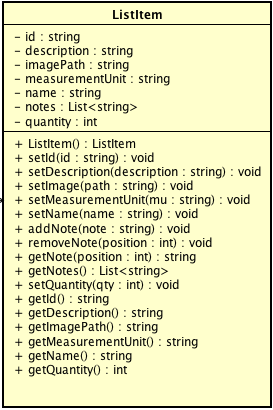
\includegraphics[scale=0.5]{Sezioni/SottosezioniST/img/app/ListItem.png}
	\caption{list\_data::ListItem}
\end{figure}

\begin{itemize}
\item \textbf{Descrizione}: Questa classe rappresenta i prodotti della lista-spesa.
\item \textbf{Utilizzo}: Viene utilizzata da tutte le classi che hanno a che fare con i prodotti della lista, ovvero che aggiungono, rimuovono e modificano gli oggetti della lista.
\item \textbf{Attributi}: 
	\begin{itemize}
	\item \textit{private id:string}\\
		Questa stringa rappresenta l'identificativo del prodotto.
	\item \textit{private description:string}\\
	Questa stringa rappresenta il la descrizione del prodotto.
	\item \textit{private imagePath:string}\\
		Questa stringa rappresenta il percorso dell'immagine del prodotto.
	\item \textit{private measurementUnit:string}\\
	Questa stringa rappresenta l'unità di misura relativa alla quantità di prodotto.
	\item \textit{private name:string}\\
	Questa stringa rappresenta il nome del prodotto.
	\item \textit{private notes:List<string>}\\
	Questa stringa rappresenta le note relative al prodotto.
	\item \textit{private quantity:int}\\
	Questa stringa rappresenta la quantità di prodotto richiesta.
	\end{itemize}
\item \textbf{Metodi}:
	\begin{itemize}
	\item \textit{public ListItem():ListItem}\\
	Il costruttore della classe ListItem.
	\item \textit{public setId(id:string):void}\\
	Imposta l'id del prodotto.
				\item{\textbf{Parametri}: \begin{itemize}
				\item \textit{id:string}\\
						L'id che verrà impostato per il prodotto.
			\end{itemize}}
	\item \textit{public setDescription(description:string):void}\\
	Imposta la descrizione del prodotto.
				\item{\textbf{Parametri}: \begin{itemize}
				\item \textit{description:string}\\
				La descrizione relativa al prodotto.
			\end{itemize}}
	\item \textit{public setImage(path:string):void}\\
	Imposta l'immagine al prodotto.
				\item{\textbf{Parametri}: \begin{itemize}
				\item \textit{path:string}\\
				l percorso dell'immagine che verrà impostata per il prodotto.
			\end{itemize}}
	\item \textit{public setMeasurementsUnit(mu:string):void}\\
	Imposta l'unità di misura relativa alla quantità di prodotto.
				\item{\textbf{Parametri}: \begin{itemize}
				\item \textit{mu:string}\\
				L'unità di misura che verrà impostata al prodotto.
			\end{itemize}}
	\item \textit{public setName(name:string):void}\\
	Imposta il nome del prodotto.
				\item{\textbf{Parametri}: \begin{itemize}
				\item \textit{name:string}\\
				Il nome che verrà impostato al prodotto.
			\end{itemize}}

	\item \textit{public addNote(note:string):void}\\
	Imposta le note relative al prodotto.
				\item{\textbf{Parametri}: \begin{itemize}
				\item \textit{note:string}\\
				Le note relative al prodotto che verranno impostate al prodotto.
			\end{itemize}}
	\item \textit{public removeNote(position:int):void}\\
	Rimuove delle note relative al prodotto.
				\item{\textbf{Parametri}: \begin{itemize}
				\item \textit{position:int}\\
				L'indice della nota da rimuovere.
			\end{itemize}}
	\item \textit{public getNote(position:int):string}\\
	Restituisce la nota relativa al prodotto nella posizione indicata.
				\item{\textbf{Parametri}: \begin{itemize}
				\item \textit{position:int}\\
				L'indice della nota di cui si vuole recuperare il contenuto.
			\end{itemize}}
	\item \textit{public getNotes():List<string>}\\
	Restituisce tutte le note relative al prodotto.
	\item \textit{public setQuantity(qty:int):void}\\
	Imposta la quantità richiesta di prodotto.
				\item{\textbf{Parametri}: \begin{itemize}
				\item \textit{qty:int}\\
				Quantità che verrà impostata al prodotto.
			\end{itemize}}
	\item \textit{public getId():string}\\
	Restituisce l'id del prodotto.
	\item \textit{public getImagePath():string}\\
	Restituisce il percorso dell'immagine del prodotto.
	\item \textit{public getName():string}\\
	Restituisce il nome del prodotto.
	\item \textit{public getDescription():string}\\
	Restituisce la descrizione del prodotto.
	\item \textit{public getMeasurementUnit():string}\\
	Restituisce l'unità di misura impostata al prodotto.
	\item \textit{public getQuantity():int}\\
	Restituisce la quantità di prodotto richiesta.
\end{itemize}
\item \textbf{Eventi}:
\end{itemize}